\chapter{引言}\label{ch:background}

% 选题背景:说明课程设计课题的目的与意义、应解决的主要问题及应达到的技术要求;
% 简述研究与发展概况及存在的问题,本设计的指导思想
\section{课题背景与意义}\label{sec:purpose}

\subsection{课题背景}
编译器(Compiler)是一种计算机程序,它会将某种编程语言写成的源代码(原始语言)
转换成另一种编程语言(目标语言)。
它主要的目的是将便于人编写、阅读、维护的高级计算机语言所写作的源代码程序,
翻译为计算机能解读、运行的低阶机器语言的程序,也就是可执行文件。

编译器将原始程序(Source program)作为输入,翻译产生使用目标语言(Target language)的等价程序。
源代码一般为高级语言(High-level language),如Pascal、C、C++、Java等,
而目标语言则是汇编语言或目标机器的目标代码(Object code),有时也称作机器代码(Machine code)。

早期的计算机软件都是用汇编语言直接编写的,这种状况持续了数年。
当人们发现为不同类型的中央处理器(CPU)编写可重用软件的开销要明显高于编写编译器时,
人们发明了高级编程语言。由于早期的计算机的内存很少,当大家实现编译器时,遇到了许多技术难题。

逐渐地,编译技术成熟了起来,高级语言在许多领域流行也起来。由于新的编程语言支持的功能越来越多,
计算机的架构越来越复杂,这使得编译器也越来越复杂。

早期的编译器是用汇编语言编写的。
首个能编译自己源程序的编译器是在1962年由麻省理工学院的Hart和Levin制作的。
从20世纪70年代起,实现能编译自己源程序的编译器变得越来越可行,
不过还是用Pascal和C语言来实现编译器更加流行。

\autoref{fig:compiler_process}中给出了一个现代编译器完整的工作流程。
其中,本次课题主要研究的是其中{\bf 编译器}的部分,也即俗称的编译器的{\bf 前端}。
主要实现了{\bf 词法分析}和{\bf 语法分析}。

\begin{figure}[hbt]
	\centering
\begin{tikzpicture}[font={\sf \small}]
	\def\smbwd{2cm}

	\node (terminal1) at (0,0) [draw, terminal,
	minimum width=\smbwd,
	minimum height=0.5cm] {源代码};

	\node (predproc1) at (0,-1.5) [draw, storage, align=left,
	minimum width=\smbwd,
	minimum height=1cm] {预处理器};

	\node (decide1) at (0,-3.5) [draw, decision,
  minimum width=\smbwd,
  minimum height=1cm] {编译器};

  \node (storage1) at (0,-5.5) [draw, storage,
  minimum width=\smbwd,
  minimum height=1cm] {汇编程序};

  \node (process1) at (0,-7.25) [draw, storage,
  minimum width=\smbwd,
  minimum height=1cm] {目标代码};

  \node (terminal2) at (0,-9.0) [draw, storage,
  minimum width=\smbwd,
  minimum height=1cm] {链接器};

  \node (terminal3) at (0,-10.5) [draw, terminal,
  minimum width=\smbwd,
  minimum height=0.5cm] {可执行文件};

  \draw[->] (terminal1) -- (predproc1);
  \draw[->] (predproc1) -- (decide1);
  \draw[->] (decide1) --  (storage1);
  \draw[->] (storage1) -- (process1);
  \draw[->] (process1) -- (terminal2);
  \draw[->] (terminal2) -- (terminal3);
\end{tikzpicture}
\caption{现代编译器工作主要流程}\label{fig:compiler_process}
\end{figure}

\subsection{课题意义}

由于高级语言根据程序员的需求变得越来越复杂,因此编译器也随之变得越来越复杂。
著名开源编译器项目LLVM的前端Clang源代码就多达336MB。\footnote{共包含源文件15034个,共有代码1756797行}
其中用到的数据结构数不胜数,各种优化方法也是层出不穷。可以说,对编译器对研究是计算机科学
中最为重要的一个研究领域,可谓皇冠上的明珠。

\section{国内外研究现状}

 众多的编译算法,包括词法分析、类型检查和推导、数据流分析、基于数据依赖性分析的循环变换、
 基于图着色的寄存器分配以及软件流水等,都是计算机科学中的奇葩。
 通过集成到各种功能强大而应用广泛的工具中,这些方法极大地影响着计算领域的实践。
 与早期的编译器实现相比,今天的编译算法明显变得越来越复杂。

 受益于基于自动机理论的词法和语法分析技术的系统化理论的发展,编译器的前端有了更加
 系统化、自动化的开发方式。因此,目前对于编译器的研究重点不再是如何实现,
 而是在于{\bf 性能}与{\bf 安全性}的提升。\cite{Advanced-compiler-optim,53e9b0b2b7602d9703b20db9}

\section{课程设计的主要研究工作}

\subsection{任务提炼}

正如\autoref{sec:purpose}所述,本次任务的主要目的是实现一个编译器的前端。
因此,我将本次任务分为以下几个步骤:

\begin{enumerate}
  \item 根据给出的要求,使用巴克斯(BNF)范式定义高级语言的词法规则、语法规则。
  \item 根据定义的词法规则,编写词法分析器。
  \item 根据定义的语法规则,编写语法分析器。
  \item 对编译器进行性能上的优化。
  \item 对编译器进行完善的测试(包括正确性测试以及错误处理测试)。
  \item 总结整个任务的完成情况,并展望未来可以提高的方面。
\end{enumerate}

\subsection{任务分析}

\paragraph{定义语言的巴克斯范式}

巴克斯范式是一种用于表示上下文无关文法的语言,上下文无关文法描述了一类形式语言,
它更广泛地使用于程序设计语言、指令集、通信协议的语法表示中。
通过巴克斯范式,我们能够精确、直观地定义语言的组成部分
(例如:{\it 标识符、数字、关键字、语句构成等})。
从而才能编写词法分析器与语法分析器,因此我们首先需要严格规定我们编译器所针对的语言,
才能更好的进行接下来的步骤。

\paragraph{词法分析}

词法分析部分是整个任务的基础,也是编译器能识别源文件的关键。词法分析通过有限自动状态机
(FSA)进行分词(tokenize),将源文件(视为文本)根据空格、换行等分隔符划分为
一个个词(token)。\autoref{fig:lex_FSM}中给出了有限自动状态机的部分定义
(没有包括全部关键词和运算符)。

\begin{figure}[hbt]
  \centering
  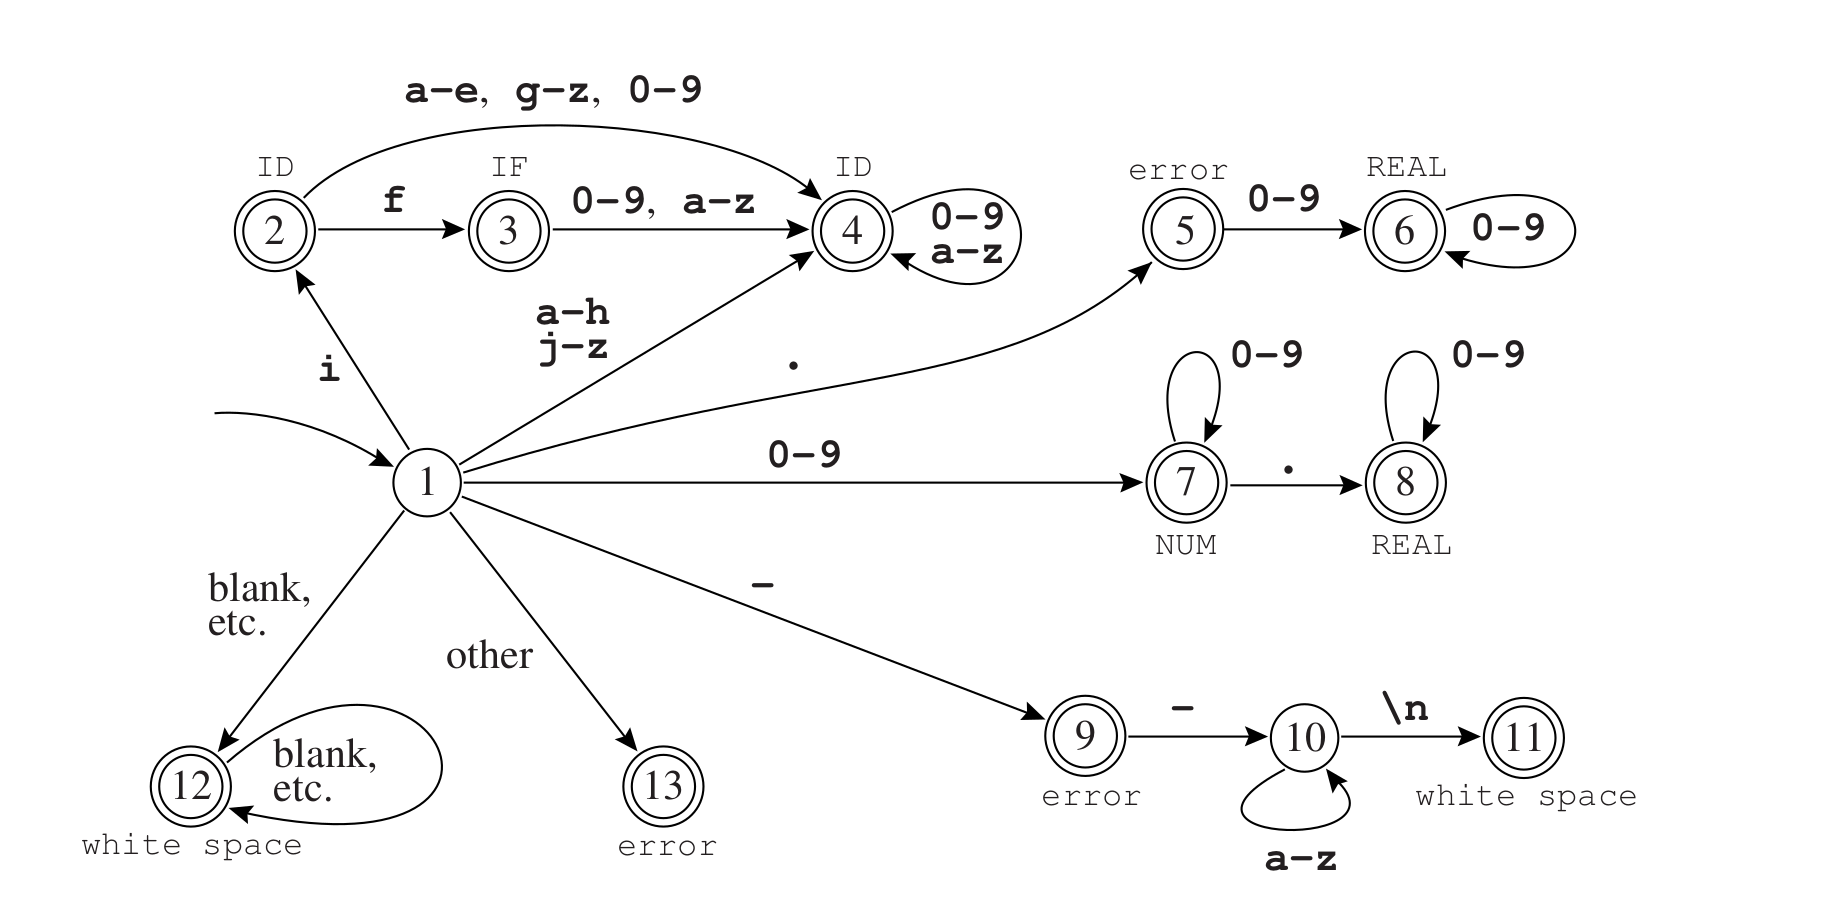
\includegraphics[scale=.25]{FSM1.png}
  \caption{词法分析有限自动状态机}\label{fig:lex_FSM}
\end{figure}

\paragraph{语法分析}

经过了词法分析后,编译器已经能够识别源文件中每一个语素是什么了,但是还不清楚它们组合起来是什么意思。
于是我们就要进行语法分析,根据定义的巴克斯范式,分析我们的语素是否组合正确。
在本次任务中,我选择使用较为简单的递归下降(Recursive descent)算法来进行词法分析。
\cite{53e9b0b2b7602d9703b20db9,Recursive-programming,appel2004modern,muchnick1997advanced,aho1986compilers}

递归下降算法是一种自顶向下的解析器,用于解析LL语法\cite{aho1986compilers}。
需要编写一组相互递归调用的过程,其中每个过程都实现了一部分都语法内容。
最终语法分析器的结构会与所定义的语法紧密相连。
\autoref{fig:recursive-decent}给出了一个简单的递归下降生成语法树的例子。

\begin{figure}[hbt]
  \centering
  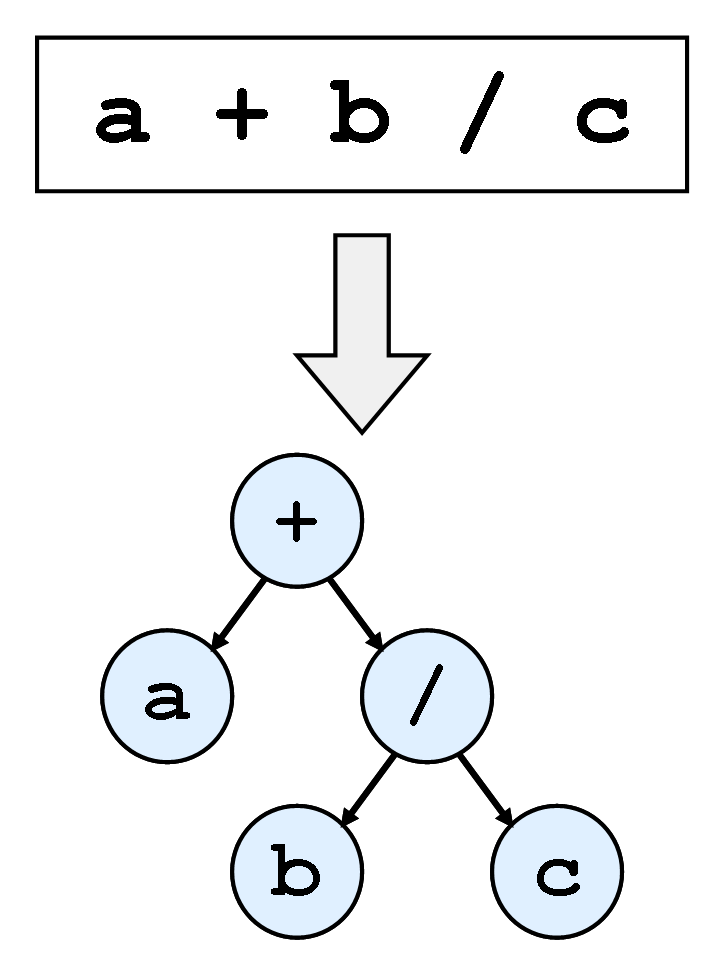
\includegraphics[scale=.4]{recursive-decent.png}
  \caption{递归下降简单示例}\label{fig:recursive-decent}
\end{figure}

通过语法分析,编译器能够完全了解源文件所想表达的含义,从而也就能够生成
{\bf\it 抽象语法树}(AST)。至此,编译器前端的任务就已经完成了,
编译器的后端会根据前端提供的抽象语法树来生成目标代码。
\footnote{因此现在创建一个编程语言变得容易了很多,如rust、swift都是站在了LLVM的肩膀上,
自己负责前端的词法分析和语法分析,将生成代码交给更专业、优化更精细的LLVM。}
